% !TEX root=/home/tavant/these/manuscript/src/manuscript.tex

\section{Presentation of the Axial-azimuthal simulation}


Here we present the Z-theta simulation domain.


\begin{figure}[hbt]
  \centering
  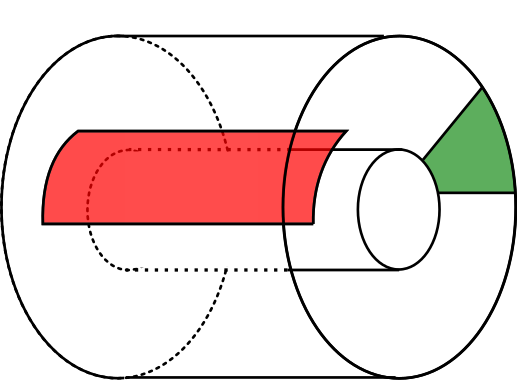
\includegraphics[width=\defaultwidth]{3D_shematic}
  \caption{Schematic representation of the chamber of a \ac{HET} and (green) the Radial-azimuthal and (red) the axial-azimuthal 2D simulation domains.}
  \label{fig-3Dschematic}
\end{figure}

\subsection{Dealing with the breathing mode} \label{subsec-breathmod}
\inlinenote{Anne: reformuler un peu pour faire apparaitre que la difficulté vient des echelles de temps et d'espace très différentes entre notamment l'ECDI et le breathing mode.}
The breathing mode comes from the coupling between the neutral gas flow, the plasma dynamics and the ionization.
Hence, if the ionization and the neutral gas are self-consistently modeled, the mean neutral density will oscillates with a frequency of about $10$ kHz.
If these oscillations are not problematic to simulate in fluid or \ac{DK} simulations, they are for particular simulations.
\inlinenote{Anne: quand tu dis "oscillates", je pense qu'il faut donner un chiffre pour montrer que ce ne sont pas juste des "petites oscillations".}
\inlinenote{Anne: euh en DK a mon avis, ca prendrait trop de temps a simuler...}

Indeed, the total number of numerical particles is proportional to the mean plasma density, and a minimal number of particles is required to limit the numerical heating \citep{turner2006}.
Thus, when the mean plasma density oscillates, the number of numerical particles (hence the amount of memory used) oscillates.
This reduces significantly the performance of the simulation code, and can lead to memory overflow if the memory available is not high enough to store all of the particles during the peak of density  of the oscillation.

A method that can be used to reduce the computational load due to the oscillation is the \emph{merging-splitting} of the particles.
When too many particles are present in a cell, they are merged into fewer particles.
Respectively, if too few particles are present, they are split into more particles.
The difficulty of this method is the conservation of the particle distribution function.
For instance, merging two particles into one cannot conserve both density and momentum.
More importantly, the temperature of the particles is lost.

In addition to the number of particles, the numerical parameters (time step and cell size) have to be chosen to satisfy the stability criteria during all of the simulation, which also reduces significantly the performance of the simulation. 
This could be overcome by adapting dynamically the mesh and the time step.
However, too few studies of the consequences of the use of merging-splitting and adaptative mesh on the simulation results have been conducted.
Thus, we have chosen not to modify the current algorithm.


Two approaches have been followed:
\begin{enumerate}
  \item the approach used by \citet{coche2014}, using a scaling of the permittivity to reduce the computational load,
  \item the approach of \citet{boeuf2017}, using a forced ionization source term.
\end{enumerate} 

\paragraph{Coche's simulation case \\}

The simulation proposed by \citet{coche2014} models self-consistently the ionization with the \ac{MCC} algorithm, as well as the neutral gas flow by supposing a constant velocity.
\Cref{fig-coche-presnetation} presents the domain of simulation 
The simulation domain geometry is realistic, with a channel length $L_{chanel} = 2.5\,\centi\meter$ for a total axial length of the simulation domain $L_z=4\,\centi\meter$.
Hence, all of the chamber and a part of the near plume is simulated.

\renewcommand\subfigurewidth{0.4\textwidth}


\begin{figure}[hbt]
  \centering
  \begin{tabular}{cc}
    \subfigure{coches_domain}{}{10,10} &
    \subfigure{coches_profiles}{}{10,10} \\
  \end{tabular}
  \caption{(left) the \ac{2D} axial azimuthal domain; (right) the axial profile of the magnetic field and the initial xenon neutral gas profile used for the simulation case of Coche. }
  \label{fig-coche-presnetation}
\end{figure}

The constraints on the time step and the cell size are alleviated by using a scaling on the permittivity.
It is simply increased by a coefficient $\alpha$, as used in other low-temperature modelling \citep{fubiani2012,boeuf2012,liu2010}.
The electron plasma frequency and electron Debye length thus become (starred quantities)
\begin{equation} \label{eq-scaled_lde}
  \lde^* = \sqrt{\frac{\alpha \epsilon_0 \Te}{e n_e}} = \lde \alpha^{1/2}
\end{equation}
\begin{equation} \label{eq-scaled_wpe}
  \ope^* = \sqrt{\frac{e^2 n_e}{\alpha \epsilon_0 m_e}} = \ope \alpha^{-1/2}
\end{equation}
Hence, the constraints on the time step and the cell size are reduced by a factor $\sqrt{\alpha}$
\begin{align*}
  \Delta t ^* &= \alpha^{1/2} \Delta t \\
  \Delta x ^*&= \alpha^{1/2} \Delta x  
\end{align*}

By doing so, \citet{coche2014} successfully observed the breathing mode in the \ac{PIC}-\ac{MCC} simulation.
The value of scaling used is $\alpha=80$, which correspond to increase of $9$ on the time step and the cell size.


\paragraph{Boeuf's simulation case \\}

In \citet{boeuf2018}, the authors used a simplified simulation set-up in order to better study the azimuthal instabilities.
The simulation is collisionless and the ionization profile is not-self-consistent but  is given as an input of the model.
This allows to remove the breathing mode oscillations from the discharge, and to simplify the parametric study of the plasma density.
The simulation domain is also smaller than the usual chamber, reducing again the computational load.



\begin{figure}[hbt]
  \centering
  \begin{tabular}{cc}
    \subfigure{boeuf-domain.png}{}{10,10} &
    \subfigure{boeuf-profiles.png}{}{10,10} \\
  \end{tabular}
  \caption{(left) the \ac{2D} axial azimuthal domain; (right) the axial profile of the magnetic field and the ionization source term profiles used for the simulation case of Boeuf. }
  \label{fig-boeuf-presnetation}
\end{figure}

\inlinenote{The simulation models (boundary conditions and so on) need to be given. See the publications (Thomas' and Boeuf's)}

\subsection{Model for radial losses} \label{subsec-fakeR}

In this section, we discuss the objective to add to the purely \ac{2D} axial-azimuthal \ac{PIC} simulation the impact of the radial walls.
The first effect that we want to model is the particle and power losses to the wall.
Thus, as previously done in the radial-azimuthal simulation, the particles are tracked in the three directions.
A finite radial length is used to limit the radial direction.
To begin with, we do not model the secondary electron emission.

When an ion crosses the boundary, it is removed from the simulation.
The electrons should be reflected by a sheath that results in an electron flux absorbed at the wall equal to the ion flux.
We suppose that the sheath is infinitely thin, so that the wall corresponds to a partially reflecting surface.
Two approaches have been investigated to model efficiently the effect of the sheath.


\paragraph{ Model 1 for the radial losses\string: sheath model\\}
The first approach set the potential drop at the walls by using  a sheath model, such as the one in \cref{sec-sheath}, or in \cref{ch-3,ch-4}.
The ions would be absorbed by the radial boundary, as well as the electrons of energy higher than the sheath potential.
Electrons with smaller energy are reflected spectacularly.

This model is more physical, but it would allow local charge imbalance.
Moreover, as there is no electric field self-consistently computed in the radial direction, the plasma cannot react to such imbalances.
Hence, we chose not to use it.

\paragraph{Model 1 for the  radial losses\string: flux equality\\}
The second approach directly imposes the flux equality by absorbing every time step the same number of electrons as ions.
The electrons crossing the radial boundaries are sorted by their energy, and the electrons absorbed are the most energetic ones.
The others are reflected elastically.
Due to the small number of ions crossing the boundary, and for performance issues, we choose to impose the flux equality averaged over the domain of a CPU.
As 360 CPU domains are used to decompose the whole simulation domain, this allows a partial locality of the flux equality. 
\vspace{1ex}
While the sheath can be supposed infinitely fin, the ion flux to the wall depends on the pre-sheaths, which usually display an ambipolar electric field that accelerates the ions to the ion sound speed at the sheath edge.
Since the development and validation of a pre-sheath electric field in the radial model required more resources than available, there is no such pre-sheath model present in the results presented in this chapter.
Consequently, the ion flux to the wall is a thermal flux, which is much smaller than the flux created by a pre-sheath.
Hence, using a realistic radial length  of the order of 1 or $2\,\centi\meter$, the particle losses are underestimated.
One solution is to reduce the radial length, so that the particle flux are closer to physical losses.

In the results given in the next sections are obtained with modeling the radial losses in all of the simulation domain.
This is done in order not to introduce a discontinuity, as well as to increase the impact of the radial losses on the simulation results.
